
%% bare_jrnl.tex
%% V1.3
%% 2007/01/11
%% by Michael Shell
%% see http://www.michaelshell.org/
%% for current contact information.
%%
%% This is a skeleton file demonstrating the use of IEEEtran.cls
%% (requires IEEEtran.cls version 1.7 or later) with an IEEE journal paper.
%%
%% Support sites:
%% http://www.michaelshell.org/tex/ieeetran/
%% http://www.ctan.org/tex-archive/macros/latex/contrib/IEEEtran/
%% and
%% http://www.ieee.org/



% *** Authors should verify (and, if needed, correct) their LaTeX system  ***
% *** with the testflow diagnostic prior to trusting their LaTeX platform ***
% *** with production work. IEEE's font choices can trigger bugs that do  ***
% *** not appear when using other class files.                            ***
% The testflow support page is at:
% http://www.michaelshell.org/tex/testflow/


%%*************************************************************************
%% Legal Notice:
%% This code is offered as-is without any warranty either expressed or
%% implied; without even the implied warranty of MERCHANTABILITY or
%% FITNESS FOR A PARTICULAR PURPOSE! 
%% User assumes all risk.
%% In no event shall IEEE or any contributor to this code be liable for
%% any damages or losses, including, but not limited to, incidental,
%% consequential, or any other damages, resulting from the use or misuse
%% of any information contained here.
%%
%% All comments are the opinions of their respective authors and are not
%% necessarily endorsed by the IEEE.
%%
%% This work is distributed under the LaTeX Project Public License (LPPL)
%% ( http://www.latex-project.org/ ) version 1.3, and may be freely used,
%% distributed and modified. A copy of the LPPL, version 1.3, is included
%% in the base LaTeX documentation of all distributions of LaTeX released
%% 2003/12/01 or later.
%% Retain all contribution notices and credits.
%% ** Modified files should be clearly indicated as such, including  **
%% ** renaming them and changing author support contact information. **
%%
%% File list of work: IEEEtran.cls, IEEEtran_HOWTO.pdf, bare_adv.tex,
%%                    bare_conf.tex, bare_jrnl.tex, bare_jrnl_compsoc.tex
%%*************************************************************************

% Note that the a4paper option is mainly intended so that authors in
% countries using A4 can easily print to A4 and see how their papers will
% look in print - the typesetting of the document will not typically be
% affected with changes in paper size (but the bottom and side margins will).
% Use the testflow package mentioned above to verify correct handling of
% both paper sizes by the user's LaTeX system.
%
% Also note that the "draftcls" or "draftclsnofoot", not "draft", option
% should be used if it is desired that the figures are to be displayed in
% draft mode.
%
\documentclass[journal]{IEEEtran}
%
% If IEEEtran.cls has not been installed into the LaTeX system files,
% manually specify the path to it like:
% \documentclass[journal]{../sty/IEEEtran}





% Some very useful LaTeX packages include:
% (uncomment the ones you want to load)


% *** MISC UTILITY PACKAGES ***
%
%\usepackage{ifpdf}
% Heiko Oberdiek's ifpdf.sty is very useful if you need conditional
% compilation based on whether the output is pdf or dvi.
% usage:
% \ifpdf
%   % pdf code
% \else
%   % dvi code
% \fi
% The latest version of ifpdf.sty can be obtained from:
% http://www.ctan.org/tex-archive/macros/latex/contrib/oberdiek/
% Also, note that IEEEtran.cls V1.7 and later provides a builtin
% \ifCLASSINFOpdf conditional that works the same way.
% When switching from latex to pdflatex and vice-versa, the compiler may
% have to be run twice to clear warning/error messages.





\usepackage{comment}
% *** CITATION PACKAGES ***
%
%\usepackage{natbib}
\usepackage{cite}
% cite.sty was written by Donald Arseneau
% V1.6 and later of IEEEtran pre-defines the format of the cite.sty package
% \cite{} output to follow that of IEEE. Loading the cite package will
% result in citation numbers being automatically sorted and properly
% "compressed/ranged". e.g., [1], [9], [2], [7], [5], [6] without using
% cite.sty will become [1], [2], [5]--[7], [9] using cite.sty. cite.sty's
% \cite will automatically add leading space, if needed. Use cite.sty's
% noadjust option (cite.sty V3.8 and later) if you want to turn this off.
% cite.sty is already installed on most LaTeX systems. Be sure and use
% version 4.0 (2003-05-27) and later if using hyperref.sty. cite.sty does
% not currently provide for hyperlinked citations.
% The latest version can be obtained at:
% http://www.ctan.org/tex-archive/macros/latex/contrib/cite/
% The documentation is contained in the cite.sty file itself.






% *** GRAPHICS RELATED PACKAGES ***
%
\ifCLASSINFOpdf
   \usepackage[pdftex]{graphicx}
  % declare the path(s) where your graphic files are
  % \graphicspath{{../pdf/}{../jpeg/}}
  % and their extensions so you won't have to specify these with
  % every instance of \includegraphics
  % \DeclareGraphicsExtensions{.pdf,.jpeg,.png}
\else
  % or other class option (dvipsone, dvipdf, if not using dvips). graphicx
  % will default to the driver specified in the system graphics.cfg if no
  % driver is specified.
   \usepackage[dvips]{graphicx}
  % declare the path(s) where your graphic files are
  % \graphicspath{{../eps/}}
  % and their extensions so you won't have to specify these with
  % every instance of \includegraphics
  % \DeclareGraphicsExtensions{.eps}
\fi
% graphicx was written by David Carlisle and Sebastian Rahtz. It is
% required if you want graphics, photos, etc. graphicx.sty is already
% installed on most LaTeX systems. The latest version and documentation can
% be obtained at: 
% http://www.ctan.org/tex-archive/macros/latex/required/graphics/
% Another good source of documentation is "Using Imported Graphics in
% LaTeX2e" by Keith Reckdahl which can be found as epslatex.ps or
% epslatex.pdf at: http://www.ctan.org/tex-archive/info/
%
% latex, and pdflatex in dvi mode, support graphics in encapsulated
% postscript (.eps) format. pdflatex in pdf mode supports graphics
% in .pdf, .jpeg, .png and .mps (metapost) formats. Users should ensure
% that all non-photo figures use a vector format (.eps, .pdf, .mps) and
% not a bitmapped formats (.jpeg, .png). IEEE frowns on bitmapped formats
% which can result in "jaggedy"/blurry rendering of lines and letters as
% well as large increases in file sizes.
%
% You can find documentation about the pdfTeX application at:
% http://www.tug.org/applications/pdftex



\usepackage{tikz}
\usetikzlibrary{arrows.meta,shapes,shadows,arrows,decorations.pathreplacing,decorations.markings}
\usepackage{longtable}
\usepackage{tabularx}
\usepackage{multicol}
% *** MATH PACKAGES ***
%
\usepackage[cmex10]{amsmath}
% A popular package from the American Mathematical Society that provides
% many useful and powerful commands for dealing with mathematics. If using
% it, be sure to load this package with the cmex10 option to ensure that
% only type 1 fonts will utilized at all point sizes. Without this option,
% it is possible that some math symbols, particularly those within
% footnotes, will be rendered in bitmap form which will result in a
% document that can not be IEEE Xplore compliant!
%
% Also, note that the amsmath package sets \interdisplaylinepenalty to 10000
% thus preventing page breaks from occurring within multiline equations. Use:
%\interdisplaylinepenalty=2500
% after loading amsmath to restore such page breaks as IEEEtran.cls normally
% does. amsmath.sty is already installed on most LaTeX systems. The latest
% version and documentation can be obtained at:
% http://www.ctan.org/tex-archive/macros/latex/required/amslatex/math/





% *** SPECIALIZED LIST PACKAGES ***
%
%\usepackage{algorithmic}
% algorithmic.sty was written by Peter Williams and Rogerio Brito.
% This package provides an algorithmic environment fo describing algorithms.
% You can use the algorithmic environment in-text or within a figure
% environment to provide for a floating algorithm. Do NOT use the algorithm
% floating environment provided by algorithm.sty (by the same authors) or
% algorithm2e.sty (by Christophe Fiorio) as IEEE does not use dedicated
% algorithm float types and packages that provide these will not provide
% correct IEEE style captions. The latest version and documentation of
% algorithmic.sty can be obtained at:
% http://www.ctan.org/tex-archive/macros/latex/contrib/algorithms/
% There is also a support site at:
% http://algorithms.berlios.de/index.html
% Also of interest may be the (relatively newer and more customizable)
% algorithmicx.sty package by Szasz Janos:
% http://www.ctan.org/tex-archive/macros/latex/contrib/algorithmicx/




% *** ALIGNMENT PACKAGES ***
%
\usepackage{array}
% Frank Mittelbach's and David Carlisle's array.sty patches and improves
% the standard LaTeX2e array and tabular environments to provide better
% appearance and additional user controls. As the default LaTeX2e table
% generation code is lacking to the point of almost being broken with
% respect to the quality of the end results, all users are strongly
% advised to use an enhanced (at the very least that provided by array.sty)
% set of table tools. array.sty is already installed on most systems. The
% latest version and documentation can be obtained at:
% http://www.ctan.org/tex-archive/macros/latex/required/tools/


%\usepackage{mdwmath}
\usepackage{mdwtab}
% Also highly recommended is Mark Wooding's extremely powerful MDW tools,
% especially mdwmath.sty and mdwtab.sty which are used to format equations
% and tables, respectively. The MDWtools set is already installed on most
% LaTeX systems. The lastest version and documentation is available at:
% http://www.ctan.org/tex-archive/macros/latex/contrib/mdwtools/


% IEEEtran contains the IEEEeqnarray family of commands that can be used to
% generate multiline equations as well as matrices, tables, etc., of high
% quality.


\usepackage{eqparbox}
% Also of notable interest is Scott Pakin's eqparbox package for creating
% (automatically sized) equal width boxes - aka "natural width parboxes".
% Available at:
% http://www.ctan.org/tex-archive/macros/latex/contrib/eqparbox/





% *** SUBFIGURE PACKAGES ***
\usepackage[tight,footnotesize]{subfigure}
% subfigure.sty was written by Steven Douglas Cochran. This package makes it
% easy to put subfigures in your figures. e.g., "Figure 1a and 1b". For IEEE
% work, it is a good idea to load it with the tight package option to reduce
% the amount of white space around the subfigures. subfigure.sty is already
% installed on most LaTeX systems. The latest version and documentation can
% be obtained at:
% http://www.ctan.org/tex-archive/obsolete/macros/latex/contrib/subfigure/
% subfigure.sty has been superceeded by subfig.sty.



%\usepackage[caption=false]{caption}
%\usepackage[font=footnotesize]{subfig}
% subfig.sty, also written by Steven Douglas Cochran, is the modern
% replacement for subfigure.sty. However, subfig.sty requires and
% automatically loads Axel Sommerfeldt's caption.sty which will override
% IEEEtran.cls handling of captions and this will result in nonIEEE style
% figure/table captions. To prevent this problem, be sure and preload
% caption.sty with its "caption=false" package option. This is will preserve
% IEEEtran.cls handing of captions. Version 1.3 (2005/06/28) and later 
% (recommended due to many improvements over 1.2) of subfig.sty supports
% the caption=false option directly:
%\usepackage[caption=false,font=footnotesize]{subfig}
%
% The latest version and documentation can be obtained at:
% http://www.ctan.org/tex-archive/macros/latex/contrib/subfig/
% The latest version and documentation of caption.sty can be obtained at:
% http://www.ctan.org/tex-archive/macros/latex/contrib/caption/




% *** FLOAT PACKAGES ***
%
%\usepackage{fixltx2e}
% fixltx2e, the successor to the earlier fix2col.sty, was written by
% Frank Mittelbach and David Carlisle. This package corrects a few problems
% in the LaTeX2e kernel, the most notable of which is that in current
% LaTeX2e releases, the ordering of single and double column floats is not
% guaranteed to be preserved. Thus, an unpatched LaTeX2e can allow a
% single column figure to be placed prior to an earlier double column
% figure. The latest version and documentation can be found at:
% http://www.ctan.org/tex-archive/macros/latex/base/



\usepackage{stfloats}
% stfloats.sty was written by Sigitas Tolusis. This package gives LaTeX2e
% the ability to do double column floats at the bottom of the page as well
% as the top. (e.g., "\begin{figure*}[!b]" is not normally possible in
% LaTeX2e). It also provides a command:
%\fnbelowfloat
% to enable the placement of footnotes below bottom floats (the standard
% LaTeX2e kernel puts them above bottom floats). This is an invasive package
% which rewrites many portions of the LaTeX2e float routines. It may not work
% with other packages that modify the LaTeX2e float routines. The latest
% version and documentation can be obtained at:
% http://www.ctan.org/tex-archive/macros/latex/contrib/sttools/
% Documentation is contained in the stfloats.sty comments as well as in the
% presfull.pdf file. Do not use the stfloats baselinefloat ability as IEEE
% does not allow \baselineskip to stretch. Authors submitting work to the
% IEEE should note that IEEE rarely uses double column equations and
% that authors should try to avoid such use. Do not be tempted to use the
% cuted.sty or midfloat.sty packages (also by Sigitas Tolusis) as IEEE does
% not format its papers in such ways.


%\ifCLASSOPTIONcaptionsoff
%  \usepackage[nomarkers]{endfloat}
% \let\MYoriglatexcaption\caption
% \renewcommand{\caption}[2][\relax]{\MYoriglatexcaption[#2]{#2}}
%\fi
% endfloat.sty was written by James Darrell McCauley and Jeff Goldberg.
% This package may be useful when used in conjunction with IEEEtran.cls'
% captionsoff option. Some IEEE journals/societies require that submissions
% have lists of figures/tables at the end of the paper and that
% figures/tables without any captions are placed on a page by themselves at
% the end of the document. If needed, the draftcls IEEEtran class option or
% \CLASSINPUTbaselinestretch interface can be used to increase the line
% spacing as well. Be sure and use the nomarkers option of endfloat to
% prevent endfloat from "marking" where the figures would have been placed
% in the text. The two hack lines of code above are a slight modification of
% that suggested by in the endfloat docs (section 8.3.1) to ensure that
% the full captions always appear in the list of figures/tables - even if
% the user used the short optional argument of \caption[]{}.
% IEEE papers do not typically make use of \caption[]'s optional argument,
% so this should not be an issue. A similar trick can be used to disable
% captions of packages such as subfig.sty that lack options to turn off
% the subcaptions:
% For subfig.sty:
% \let\MYorigsubfloat\subfloat
% \renewcommand{\subfloat}[2][\relax]{\MYorigsubfloat[]{#2}}
% For subfigure.sty:
% \let\MYorigsubfigure\subfigure
% \renewcommand{\subfigure}[2][\relax]{\MYorigsubfigure[]{#2}}
% However, the above trick will not work if both optional arguments of
% the \subfloat/subfig command are used. Furthermore, there needs to be a
% description of each subfigure *somewhere* and endfloat does not add
% subfigure captions to its list of figures. Thus, the best approach is to
% avoid the use of subfigure captions (many IEEE journals avoid them anyway)
% and instead reference/explain all the subfigures within the main caption.
% The latest version of endfloat.sty and its documentation can obtained at:
% http://www.ctan.org/tex-archive/macros/latex/contrib/endfloat/
%
% The IEEEtran \ifCLASSOPTIONcaptionsoff conditional can also be used
% later in the document, say, to conditionally put the References on a 
% page by themselves.





% *** PDF, URL AND HYPERLINK PACKAGES ***
%
\usepackage{url}
% url.sty was written by Donald Arseneau. It provides better support for
% handling and breaking URLs. url.sty is already installed on most LaTeX
% systems. The latest version can be obtained at:
% http://www.ctan.org/tex-archive/macros/latex/contrib/misc/
% Read the url.sty source comments for usage information. Basically,
% \url{my_url_here}.





% *** Do not adjust lengths that control margins, column widths, etc. ***
% *** Do not use packages that alter fonts (such as pslatex).         ***
% There should be no need to do such things with IEEEtran.cls V1.6 and later.
% (Unless specifically asked to do so by the journal or conference you plan
% to submit to, of course. )


% correct bad hyphenation here
\hyphenation{op-tical net-works semi-conduc-tor}

\pagestyle{empty}

\begin{document}
%
% paper title
% can use linebreaks \\ within to get better formatting as desired
\title{THEORITICAL PREDICTION AND MATHEMATICAL FORMUALTION OF THE MATERIAL  COMPOSITION FOR MICROWAVE ABSORPTION APPLICATIONS}
%
%
% author names and IEEE memberships
% note positions of commas and nonbreaking spaces ( ~ ) LaTeX will not break
% a structure at a ~ so this keeps an author's name from being broken across
% two lines.
% use \thanks{} to gain access to the first footnote area
% a separate \thanks must be used for each paragraph as LaTeX2e's \thanks
% was not built to handle multiple paragraphs
%

\author{Aayushi Arya,Dr GVV Sharma}
%,~\IEEEmembership{Member,~IEEE,}
 %      John~Doe,~\IEEEmembership{Fellow,~OSA,}
  %    and~Jane~Doe,~\IEEEmembership{Life~Fellow,~IEEE}% <-this % stops a space
%  \author{AayushiArya}
%\thanks{M. Shell is with the Department
%of Electrical and Computer Engineering, Georgia Institute of Technology, Atlanta,
%GA, 30332 USA e-mail: (see http://www.michaelshell.org/contact.html).}% <-this % stops a space
%\thanks{J. Doe and J. Doe are with Anonymous University.}% <-this % stops a space
%\thanks{Manuscript received April 19, 2005; revised January 11, 2007.}}

% note the % following the last \IEEEmembership and also \thanks - 
% these prevent an unwanted space from occurring between the last author name
% and the end of the author line. i.e., if you had this:
% 
% \author{....lastname \thanks{...} \thanks{...} }
%                     ^------------^------------^----Do not want these spaces!
%
% a space would be appended to the last name and could cause every name on that
% line to be shifted left slightly. This is one of those "LaTeX things". For
% instance, "\textbf{A} \textbf{B}" will typeset as "A B" not "AB". To get
% "AB" then you have to do: "\textbf{A}\textbf{B}"
% \thanks is no different in this regard, so shield the last } of each \thanks
% that ends a line with a % and do not let a space in before the next \thanks.
% Spaces after \IEEEmembership other than the last one are OK (and needed) as
% you are supposed to have spaces between the names. For what it is worth,
% this is a minor point as most people would not even notice if the said evil
% space somehow managed to creep in.



% The paper headers
\markboth{Journal of \LaTeX\ Class Files,~Vol.~6, No.~1, January~2007}%
{Shell \MakeLowercase{\textit{et al.}}: Bare Demo of IEEEtran.cls for Journals}
% The only time the second header will appear is for the odd numbered pages
% after the title page when using the twoside option.
% 
% *** Note that you probably will NOT want to include the author's ***
% *** name in the headers of peer review papers.                   ***
% You can use \ifCLASSOPTIONpeerreview for conditional compilation here if
% you desire.




% If you want to put a publisher's ID mark on the page you can do it like
% this:
%\IEEEpubid{0000--0000/00\$00.00~\copyright~2007 IEEE}
% Remember, if you use this you must call \IEEEpubidadjcol in the second
% column for its text to clear the IEEEpubid mark.



% use for special paper notices
%\IEEEspecialpapernotice{(Invited Paper)}



\maketitle
\thispagestyle{empty}


\begin{abstract}
%\boldmath
Microwave Absorbers has become an essential requirement in various fields including industrial uses like Radar, Stealth , commercial uses in mobile networking , EMI , EMC, electronic toll collection, social applications like in hospitals , schools , where the microwave flux has crossed the threshold. In the past few years, there has been  an intense experimental work to explore various materials for the different applications , focusssing on their effectiveness, stability. The hit and trial cycles of the experimentation can be reduced with a theoritical model predicting the suitability of material for MA applications, allowing more accurate , rigorous and wide prespective for the experimentation. Thus, in this work , an attempt has been made provide a conceptual and theoritical mathematical formulation based model to predict the suitability of various elements and their composition for specified application. The model is based on Transmission Line Theory, Polarizability, dielectric response of material. The  parameters are derived for the MA  are characteristic impedance, input impedance , permittivity , permeability polarizability , Molar refraction ratio, Polarisation Energy. Using the above paramters and the material properties like its global hardness factor, we conclude to a set of theoritical atomic radii , which can be suitable for the absorption at the specified frequency , which is 2.54 GHz ( ISM band -immensely used in various eelctronic applications). Further a composition of two or more elements viz. oxides of material, alloys , and multi cation oxides, can be predicted by comparing their spatial energy parameter , which depends on their individual valency and global hardness factor.This work is beneficial for not only understanding the fundamental molecular level perspective of the absorbers but also in providing a conceptual and engineering aspect to further explore new materials for the microwave absorption , with less error rate.
\end{abstract}
% IEEEtran.cls defaults to using nonbold math in the Abstract.
% This preserves the distinction between vectors and scalars. However,
% if the journal you are submitting to favors bold math in the abstract,
% then you can use LaTeX's standard command \boldmath at the very start
% of the abstract to achieve this. Many IEEE journals frown on math
% in the abstract anyway.

% Note that keywords are not normally used for peerreview papers.
\begin{IEEEkeywords}
EMI , Reflection Loss, Resonance, Dielectric Parameters,Polarisation Energy,Atomic Radii.
\end{IEEEkeywords}






% For peer review papers, you can put extra information on the cover
% page as needed:
% \ifCLASSOPTIONpeerreview
% \begin{center} \bfseries EDICS Category: 3-BBND \end{center}
% \fi
%
% For peerreview papers, this IEEEtran command inserts a page break and
% creates the second title. It will be ignored for other modes.
\IEEEpeerreviewmaketitle



\section{Introduction}
% The very first letter is a 2 line initial drop letter followed
% by the rest of the first word in caps.
% 
% form to use if the first word consists of a single letter:
% \IEEEPARstart{A}{demo} file is ....
% 
% form to use if you need the single drop letter followed by
% normal text (unknown if ever used by IEEE):
% \IEEEPARstart{A}{}demo file is ....
% 
% Some journals put the first two words in caps:
% \IEEEPARstart{T}{his demo} file is ....
% 
% Here we have the typical use of a "T" for an initial drop letter
% and "HIS" in caps to complete the first word.
\IEEEPARstart{M}{icrowave Absorbers} , has now become an area of  immense research for both electronic field and materials design . The immediate need of Microwave absorbers is highlighted due to their necessity in the current technological scenario. need Due to the exponential growth of the usage of high frequency  electronic hardware and wireless communication, there is a dramatical increase of the microwaves flux in the ambient surroundings , which causes ElectroMagnetic Interference amomg the underlying circuits undesirably by generating unwanted noise, cross connection ,false output etc. The critical exposure of microwaves  also has harmful effects on the health , especially for hospitals, schools and highly populated residential areas. This creates a  need to mitigate the surrounding EM wave  noise, has driven researchers to develop materials that can effectively absorb the unwanted radiations ,protecting the underneath circuitry. Various materials and their composition are investigated using experimental procedures like Vector Network Analyzer, Impedance Analyzer to test their ability as absorbers. Meanwhile , there is also ongoing work to theoritically understand and model Microwave Absorbers. There are range of wave theory based electrical, magnetic parameters associated with the working of MA.
First is the Reflection Loss and the Characteristic Impedance of a Microwave absorber that can be calculated using Transmission Line Theory \cite{YingL2}.The latter is an intrinsic property independent of the thickness of the sample.
Similar theory is applicable to ferrite based microwave absorbers conatining both electric and magnetic dipoles represnted by  permittivity and permeability respectively \cite{YingL}.The oscillations of dipoles in a MA are both resonant and non resonant. . A detailed absorption model is then provided to include all the above elements in the basics of absorption formulas of transmission line theory.

There has been also works to correlate the electrical/magnetic parameter and physical parameters of microwave absorbers. Analyising polarizability gives an insight into the wave absorbing power of a material. Following this , in \cite{Erbium} , the Lorentz-Lorenz equation was used to estimate  the electronic polarizability of ions in oxide glasses , based on their refractive indices and band gap energy.In \cite{dimitrov1999effect} , the author further discusses an Interaction Parameter for oxides based  on the polarizability of oxide ion, dtermined from the refractive index. This Parameter is used as a measure of the interionic interaction between cations and anions created due to the charge overlap of the outermost electronic orbitals.The charge overlap and the polarizability of cation and anions both affect the Interaction Parameter. This Parameter serves as an index to estimate the optical  properties of oxide glasses. Siimilarly for magnetic based microwave absorbers the magnetic dipole moment can be used as a measure for microwave absprtion.  This consecutive dependency of  properties when modelled mathematically using energy parmeter can provide a useful tool for prediction of new compositions based suitable microwave absorbing materials. The energy parameter when normalized can be directly related to the atomic radii \cite{korablev2018calculations}.
In this paper, an attempt has been made to theoritically derive the parameter related to a microwave absorber. First the transmission line theory was used to determine the electrical parameters including characteristic impedance, reflection loss, permittivity and permeability, resonance frequency . From the above paremters and a set of equations expalined below we derived  the physical parameters like polarizability, dipolar frequency . spatial energy parameter . From this we derived   the atomic range of suitable atomic radii . The compositions can be predicted by comparing the effective Energy Parameter. This approach covers all the necessary  properties required for a microwave absorber. It can be beneficial in filling the gap between the molecular and the physical properties of an absorber . It can help in predicting new compositions for efficient microwave absorbption.

\subsection{RESONANCE PARAMETERS OF MICROWAVE ABSORBERS}
Reflection Loss of a microwave absorber is given by :
\begin{equation}
 R_L(dB) = 20log|\frac{(Z_{in} - Z_o)}{(Z_{in} + Z_o)}| \label{eq1}
\end{equation}
where $ Z_{in} $  is the input impedance of the MA , which it presents at the interface to the incident EM wave, when modelled as a transmission line.$ Z_o$ is the characteristic impedance of the incident medium, which in our application is air \cite{r1} \cite{r2}.

\subsubsection{Input Impedance and Quality Factor}
Keeping Reflection loss -20 dB , which is a standard measure for 99 percent  of absorption .
Also , taking into account the free space impedance as $ Z_o = 377  $ ohm and above value of  reflection loss in equation(1) , we get the input impedance of the microwave absorber as 

\begin{align}
Z_in = 460.78 \Omega  \label{v1}
\end{align} 

 The input impedance of the microwave absorber can be written in terms of a Transmission line , with an open circuit end as \cite{YingL2}:-
 \begin{align}
 Z_(in) = Z_o \sqrt{\frac{\mu }{\epsilon}} \tanh(\frac{-j2 \pi f d \sqrt{ \mu \epsilon}}{c}) \label{eq2}
 \end{align}
 
CHARACTERISTIC IMPEDANCE OF MA:The value of characteristic impedance $Z_o $ to be used in 
ref{eq1} is derived from the net reflection loss which is -20 dB , used in the below equation \cite{Shukla}
\begin{equation}
R.L = 20 \log(\frac{Z_o}{4Z_{in}}) \label{eq3} \\
Z_o = 184 \Omega  \\
\end{equation}

The Q factor is the quality factor , which determines the damping ability of the absorber\cite{YingL2}. The Q factor, damping ratio $\zeta$ and exponential decay factor $\alpha$ are related as \cite{r5}
\begin{align}
\zeta = \frac{1}{2Q} \\
 &= \frac{\alpha}{\omega_o} \label{two}\\
 \omega_n = \sqrt{\frac{k}{m}} \label{three}
\end{align}
Quality factor is also expressed in terms of resonance frequency as \cite{r2}:
$$   Q = \dfrac{2 \pi f_r}{2 \pi \Delta f_r} \label{four} \\
           = \dfrac{\omega_r}{\delta \omega_r}
$$ where $ \omega_r$ is the resonance frequency and $\delta \omega_r$ is the bandwidth over which the absorption is greater than half of the maximum at the center frequency.
Since damping of the waves in a medium is characterised by the amount and type of absorption. Using basic damping classification , we take Q $<$ 1/2 considering it as OVERDAMPED SYSTEM \cite{r6} . corresponding to this Q value we get $$\zeta = 1.5 $$

where $\omega_n $ is the natural resonance frequency of the system. $k$ is the wave propagation constant
Using $\zeta=1.5 $ and the following equations we can deduce the values of exponential decay constant$\alpha$, natural resonant frequency of the system $\omega_o$ and the dipole relaxation time constant $\tau$. The equations are as follows:-
\begin{align}
 Q &= \dfrac{1}{2 \zeta} = \dfrac{1}{2 X damping ratio} \label{five}\\
   &= \dfrac{\alpha}{\omega_n} \label{six}\\
   &= \dfrac{1}{\tau \omega_n}
\end{align}
 Using the above equations, we get the values as:
 
%\fbox{
%\begin{minipage}[]{0.4\textwidth}
\begin{align} 
 Z_in = 460.77 \Omega \\
\zeta = 1.5  \\
Q &= \frac{1}{2 \zeta}  \\
 &=  o.33 \label{seven} \\ 
f_r = 2.54 GHz   \\
\omega_r = 1.53 X 10^{10} rad/sec \\
Q = \frac{\omega_r}{\triangle  \omega_r} \\
\triangle \omega_r = 4.83 X 10^{10} rad/sec
\end{align}
%\end{minipage}
%}
%\hfill
%\fbox{
%\begin{minipage}[t]{0.4\textwidth}

\subsubsection{Exponential Decay Factor Natural Resonant frequencyand width(d) of MA}
Using the Q as in ref{seven} value , we can calculate $ \alpha$ as 
\begin{align} 
Q &= \frac{\alpha}{\omega_0}\\
 &= \alpha = 2.39 X 10^{10} \label{polar}
\end{align}
Again using ref{seven} , we determined the natural resonance frequency that came out to be 
\begin{align*}
\omega_n = 7.25 X 10^{10}
\end{align*}
%\end{minipage}
%}
\hfill


%\fbox{
WIDTH OF Microwave absorber: WIDTH 'd' of the
 microwave absorber is set to be around quarter wavelength, 
 making it as an OPEN -CIRCUIT TRANSMISSION LINE with a reflection null \cite{Tooley}
%}

\begin{equation} \label{nine}
d  = \dfrac{c}{4 f_m \sqrt{\epsilon_r}} 
\end{equation}

%\fbox{
%\begin{minipage}{0.4\textwidth}
%\color{black}{\huge{Using the value of 'd' as in \ref{nine} in the input 
i%mpedance equation as in \ref{one} we get the value of 
%relative permittivity as $\epsilon_r$ = 0.24}}
%\end{minipage}
%}
%\hfill
%\fbox{
%\begin{minipage}[t]{0.4\textwidth}
%\textbf{

%}
%\end{minipage}
%}

%\end{large}
\subsection{LOWER LIMIT OF  PERMITTIVITY AND PERMEABILITY}

\textbf{RATIO OF $\dfrac{\mu}{\epsilon}$}
\begin{align}
R_L = 20 log_{10} |\dfrac{Z_d - Z_o}{Z_d + Z_o}| \\
R_L = 20 log_{10} \left \lvert \dfrac{\sqrt{\frac{\mu_r}{\epsilon_r}} - 1}{\sqrt{\frac{\mu_r}{\epsilon_r}} +1 } \right \rvert  \\
R_L = -20 dB \\
\underbrace{\frac{\mu_r}{\epsilon_r} = 1.5 }\\
\end{align}
\textbf{PRODUCT OF $\mu_r \epsilon_r$}
\begin{align}
Z_M = Z_o  \sqrt{\frac{\mu_r}{\epsilon_r}} (\dfrac{2 \pi \nu d \sqrt{\mu_r \epsilon_r}}{c}) \\
\end{align}
Solving , it we get 
$\underbrace{\mu_r \epsilon_r = 1.6}$
using ref{one}, we can derive the value of $\epsilon_r$ and $\mu_r$, that is the relative permittivity and permeability as:-
\fbox{
First datapoint:-
$\epsilon_r = 1.032$
$\mu = 1.55 $
}

%\subsection*{QUALITY FACTOR DETERMINATION}
%The quality factor can be deduced to 
%\begin{align}
%Q = \dfrac{4\pi}{ \omega_n} \\
%\end{align}
%at $\epsilon \mu = 1.6$, we get $Q = 0.314$ With a bandwidth of about 3 GHz, which is acceptable

\subsection{POLARIZABILITY AND RELATED PARMETRS }

The polarizability , of a material can be calculated in terms of the parameters like natural resonance frequency, operational resonance frequency , damping constant , as shown below \cite{liu2018systemized}:-

\begin{equation} \label{eight}
{\alpha}_p = \dfrac{e^2 m ({\omega_o}^2 - {\omega}^2)}{m^2({\omega_o}^2 - {\omega}^2)^2 + 4 \eta \omega^2} - \dfrac{2 e^2 \eta \omega}{m^2({\omega_o}^2 - {\omega}^2)^2 + 4 \eta \omega^2}
\end{equation}
The damping constant can be determined from the wave propagation constant k and the mass of electron m ,as given by :-
$$k = {\omega_o}^2*m$$
\begin{equation}
\eta = 2 \sqrt{km}
\end{equation}
%\fbox{
Using equation ref{eight} , we get 
$k = 2.31^{-10}$
$\eta = 2.9^{-20}$
${\alpha}_p = 2.36*10^{-28}$
%}

\subsubsection{Number of Dipoles per unit and time constant }
%\begin{large}
\begin{equation} \label{ten}
\dfrac{({\mu \epsilon})- 1}{({\mu \epsilon}) + 2 } = \dfrac{N \alpha_p}{3 \epsilon_o}
\end{equation}
This is the claussius Mosotti  equation which links the relative permittivity to the number of dipoles per unit \cite{Erbium}. Since we have reached the relative permittivity in previous section, using the above equation we get 
\fbox{
%\color{black}
$N = 1.87 X 10^{16}$
}


%\begin{minipage}[t]{0.25\textwidth}
Similarly calculating the time constant we get
%\fbox{
$ \tau= \frac{1}{\zeta \omega_o} = 8.88 X 10 ^{-12} sec$
%}

\subsubsection{Complex Permittivity and conductivity}
%\huge{
Complex Permittivity is an important electrical property of absorbing materials. It depends on resonance frequency, bandwidth, time constant as per given matematical  equations \cite{booke}.
\begin{equation}
\epsilon^{'}_{r } = \chi^{'}_{e} + 1 =
\epsilon^{'}_r = (\dfrac{\omega^2_P (\omega^2_o - \omega^2)}{(\omega^2_o - \omega^2)^2 + \frac{\omega^2}{\tau^2}}) + 1
\end{equation}
\begin{equation}
\epsilon^{''}_{r } = \dfrac{\omega^2_P (\frac{\omega}{\tau})}{(\omega^2_o - \omega^2)^2 + \frac{\omega^2}{\tau^2}}
\end{equation}
%}
Here , the value of $\omega_p $ is given as
%\color{black}{
\begin{equation}
\omega^2_p = \dfrac{n_e q^2}{\epsilon_o m}
\end{equation}
where $n_e$ is N , that is the total number of dipoles per unit volume, taking it from (ref{ten}) , 'm ' is the mass of electron . Solving above equation , we get $\omega_p$
Using the above value we can determine the natural dipolar resonant frequency as
\fbox{
$  \omega_p = 2.4 x 10^{9} rad/sec $
}

Using the parameters mentioned in above equation , are as follows
%\fbox{
%\begin{minipage}{0.25\textwidth}

\begin{align*}
N = 1.815 X 10^{15}  ~ 2 x 10^{15} \\
\omega^2_p = 6.4 X 10^{19} (rad/sec)^2 \\
\tau = 8.9 X 10^{-12} sec\\
\omega = 1.59 X 10^{10} rad/sec\\
\omega_o = 7.25 X 10^{10} rad/sec\\
\end{align*}
%\end{minipage}
%}

%\textbf{
Using these values and $ \epsilon^{''}_r = \dfrac{\sigma}{\omega \epsilon_o}$, we get
$\epsilon^{'}_r = 0.012 + 1 = 1.01 $
$\epsilon^{''}_r = 3.95X 10^{-3}$
$ \sigma = 5.29 X 10^{-4} siemens$
%}

%\end{minipage}
%\begin{minipage}[t]{0.4\textwidth}
\subsection{UPPER LIMIT OF  PERMEABILITY AND PERMITTIVITY}
%Based on the phase propagation constant as 
%$$ k_{phase} = \frac{2 \pi}{\lambda}= 53.17$$
%and the natural resonant dipolar frequency $\omega_p$, we get
%$$ n = \sqrt{\epsilon \mu} = {\dfrac{k_{phase} x c}{\omega_n}}^2$$
%which gives
%\fbox{
%$n = \sqrt{\mu \epsilon } = 6.65$
%}
Based on the below equation as 
$$ \epsilon^{''}_r  = \dfrac{n a_p c}{2 \pi \nu}$$
where $a_p = 0.1$ gives the power absorption coefficient , and n is $n = \sqrt{\epsilon \mu}$ , $\nu$ is the 
working frequency. Evaluating the above equation we get
\fbox{
$n = \sqrt{\epsilon \mu} = 2.1$
}
Permeability value can be considered by taking into account the required bandwidth , which gives the maximum damping constant value.
Further calculating the width of the MA and using the absorption formula to come to a permeability value, we can follow the previous method to attain $E_g$ and $R $ value.
%\end{minipage}
\begin{align}
d_m = \frac{1}{4}(\frac{c}{f_m \sqrt{\mu_r \epsilon_r}})   \\
\zeta_max= 2.05                                              \\
\triangle \omega_r = 6.519X 10^{10} rad/sec                   \\
{\omega_r}_+ = \omega + \frac{\triangle \omega_r}{2}            \\     
(\omega_r)_+ = 5 X ^{10} rad/sec                               \\
f_r = 7.7 GHz                                                 \\
(SE)_a = 8.7 d_{max} \sqrt{f_m \pi \mu \sigma}                  \\
\mu_r = 4.4                                                   \\
\end{align}
%$$Z_d = $$
%\end{minipage}



\subsection{POLARIZATION ENERGY, GLOBAL HARDNESS FACTOR AND THEORITICAL RADII}

%\fbox{
%\begin{minipage}[t]{0.4\textwidth}
\subsection{Polarisation Energy}
Below is the equation of the molar fraction of oxides \cite{Erbium}
$
R_m = (\dfrac{n^2_o -1}{n^2_o +2 })V_m $

$n_o$ is the linear refractive index, 
$V_m$ is the molar volume.
%}
%\end{minipage}

\hfill
%\fbox{
%\begin{minipage}[t]{0.45\textwidth}

This equation relates the polarizability to Molar refraction ratio\\
\fbox{
$
\alpha_m = \dfrac{3}{4 \pi N_A} R_M 
$\\
}
$\alpha_m$ is the polarizability as given in (ref{polar}), \\
$N_A$ is the avagadro number.\\

%\end{minipage}
%}
\

The relation between the energy gap of the oxide and the molar refraction  ratio is given by :-
\begin{equation}
E_g = 20(1- \dfrac{R_m}{V_m})^2
\end{equation}
Here , one important concept of metallization criteria should be considered which acts as a threshold for the possibility of the formation of the solid soluble compounds, M is given by

\begin{align}
M = 1 - \dfrac{R_m}{V_m}                \\
(\frac{R_m}{V_m}) < 1   NON METAL        \\
(\frac{R_m}{V_m}) < 1      METAL          \\
\end{align}
Putting all values together we get for $n = \sqrt{\epsilon_r}$

\begin{align*}
\alpha_m = 2.36 X 10^{-28} \\
R_m =  1.0 X 10^{-24}      \\
V_m = 2.95 X 10^{-24}        
\end{align*}
Ultimately
%\color{black}{
\subsubsection{R corresponding to Lower Limit}
Keeping the value we get 
%\textbf{\color{black}{
\begin{equation}
R = 0.36 \AA
\end{equation}
\begin{equation}
E_g = 19.87 eV
\end{equation}
\subsection{R corresonding to Upper Limit: Anionic}


%\begin{minipage}[t]{0.7\textwidth}
\begin{align}
E_g = 4.34 eV                                                       \\
R = 1.64 \AA                                                   \\                                    
\end{align}
\subsection{R corresonding to Upper Limit: Cationic}
Using cauchy's dispersion equations, the upper limit for the cationic radii cab be found as follows.
The electronic susceptibility can be given as :-
\begin{align}
{\chi_e}^{'} = \dfrac{\omega_p^{2}}{{\omega_o}^{2}}
\end{align}
The different constants for relating susceptibility to refractive index are:-
\begin{align}
A = 1+ \chi_e(0) = n_o^{2} \\
B = (2 \pi c)^{2}\dfrac{\chi_e(0)}{\omega_oe^{2}} \\
C = \dfrac{B}{2 A^{1/2}} \\
n = n_o + \dfrac{C}{\lambda_o^{2}} \\
n_o = \epsilon_r(0) \\
A = 4.41 \\
B= 0.012 \\
C= 3.32 X 10^{-3} \\
n= 2.34  \\
\end{align}


Radius value corresponding to the upper refractive index limit$ n=2.34$ is $ R = 2.23 \AA $
%}
\subsection{Theoritical Radii and Global hardness Factor : A COMMON DATABASE}
By evaluating a common database from an observation point of view , with regards to the elements performance towards the polarisation process. While estimating a suitable compound for EMI application , the individual elements shoud have compatible polarizing ability leading to effective absorption of the microwaves. The cations and anions should exert polarising force on each other such that there is a balanced formation of dipoles \cite{JaiS} \cite{shannon}. Below table is an effort to find easy referential parameter for comparing the suitability of various cations and anions with respect to each other. The P parameter is a measure of the overall energy characteristics of the outer orbitals taking into acoount the polarisability and the screening effect \cite{dimitrov1999electronic}. Use of this " spatial energy parameter" has already been proved in other physical phenomenons like self diffusion , as already discussed above . Improvising the given parameter to contain the information regarding the polarisation extent of the element , a set of values can be obtained for the entire set of elements providing a means to predict the compatibility of new compound formations for their EMI performance. The general formula of spatial energy parameter is \cite{korablev2018calculations}
\begin{equation}
%\dfrac{1}{\frac{q^2}{r_i}} + \dfrac{1}{E_i} = \dfrac{1}{P_E}
\dfrac{1}{{q^2}} + \dfrac{1}{\eta} = \dfrac{1}{P_o}
\end{equation}
$r_i$ is the atom orbital radius, $\eta$ is the global hardness factor,Considering the polarization energy equivalent to the Global hardness factor , which is none other than the ability of a chemical species to form bond with its neighbouring atom/molecule, as given by :-
\begin{equation}
\eta = \dfrac{e^2}{2 R}
\end{equation}
$q$ is given by below equation:-
\begin{equation}
		q = \dfrac{z^*}{n*}   
\end{equation}
\subsection{COMPUTATION OF POLARISATION ENERGY PARAMETER}

$q$ is given as the ratio of effective charge of nucleus to effective main quantum number. $q$ is affected by the screening constant of the atom which depends on the orbital exponent of the electronic orbitals \cite{clementi1963atomic} .The effective quantum number depends on the valence electron distribution among the outer orbital. It is approximated as outer orbital quantum number multiplied by total number of valence electrons in the orbital multliped by spin factor (1/2). $P_o$ is a spatial parameter indicative of overall polrisation energy . $P_E $ is the effective polarisation energy considering the atomic extent of the molecule.Using the above analogy , a database table is created where we can compare the elements based on their polarisation parameter and find their compatability to form compounds for effective microwave absorption.
Based on the parameters described above , the database was theoritically extracted to , as presented below:-

%\resizebox{0.5\textwidth}{!}{
%\begin{center}





% An example of a floating table. Note that, for IEEE style tables, the 
% \caption command should come BEFORE the table. Table text will default to
% \footnotesize as IEEE normally uses this smaller font for tables.
% The \label must come after \caption as always.
%
%\begin{table}[h!]
%% increase table row spacing, adjust to taste
%\renewcommand{\arraystretch}{1.3}
% if using array.sty, it might be a good idea to tweak the value of
% \extrarowheight as needed to properly center the text within the cells
%\caption{An Example of a Table}
%\label{table_example}
%\centering
%% Some packages, such as MDW tools, offer better commands for making tables
%% than the plain LaTeX2e tabular which is used here.
%\begin{tabular}{|c||c|}
%\hline
%One & Two\\
%\hline
%Three & Four\\
%\hline
%\end{tabular}
%\end{table}
\begin{comment}
\resizebox{0.5\textwidth}{!}{
\begin{tabular}{|c|c|c|c|c|}
\hline 
Element & Atomic Radii $\AA$ & $\eta$ & n-valency & $P_o$\\ 
\hline 
H & 0.5292 & 13.588 & 1 & 54.352 \\ 
\hline 
Li & 1.6282 & 4.4164 & 1 & 8.82	 \\ 
\hline 
Be & 1.0855 & 6.6244 & 2 & 26.5	 \\ 
\hline 
B & 0.8141 & 8.8328 & 3 /-3 & 52.99,
                              -52.99	 \\ 
\hline 
C & 0.6513 & 11.04 & +2,4 & 88.32 \\ 
\hline 
N & 0.5427 & 13.25 & +5,4,3,1 & 132.5,  106,79.5,  26.5 \\ 
\hline 
 &  &  & -1,-2,-3 & -26.5,-53,-79.5 \\ 
\hline 
O & 0.4625 & 15.46 & -2 & -61.84 \\ 
\hline 
F & 0.4071 & 17.66 & +1,-1 & =35.32,   -35.32 \\ 
\hline 
Al & • & • & • & • \\ 
\hline 
Ne & • & • & • & • \\ 
\hline 
Na & • & • & • & • \\ 
\hline 
Mg & • & • & • & • \\ 
\hline 
Al & 1.3607 & 5.2846 & +3 & 10.57 \\ 
\hline 
Si & 1.1476 & 6.27 & +4 & 50.16 \\ 
\hline 
P & 0.9922 & 7.25 & +1,+3,+5 & 14.5,  43.5,  72.5 \\ 
\hline 
    &       &      &   -3 &   -43.5 \\ 
\hline 
S & 0.8738 & 8.23  & +2,4,6  &  +32.92,   65.84,  98.76 \\ 
\hline 
   &  &    &    &  -32.92 \\ 
\hline 
Cl  & 0.7807 & 9.211 & -1,+1,+2 & -18.422,18.422,36.84  \\ 

\hline 
Ar & 0.7056 & 10.191 & 0 & 0 \\ 
\hline 
K & 3.5598 & 2.02 & +1 & 4.04 \\ 
\hline 
Ca & 2.7479 & 2.6162 & +2 & 10.46 \\ 
\hline 
Sc & 2.6106 & 2.7545 & +3 & 16.527 \\ 
\hline 
Ti & 2.486 & 2.8924 & +2,+3,+4 & 11.5696,17.35,231392 \\ 
\hline 
V & 2.3732 & 3.03 & +2,+3,+4,+5 & 12.12,18.18,24.24,30.3 \\ 
\hline 
Cr & 2.2701 & 3.1676 & +2,+3,+6 & 12.6704,19.0056,38.0112 \\ 
\hline 
Mn & 2.1754 & 3.3055 & +2,+3,+4,+6,+7 & 13.222,27.444,39.666,46.277,19.833 \\ 
\hline 
Fe & 2.20885 & 3.443 & +2,+3,+4,+6 & 13.772,27.544,41.316,20.658 \\ 
\hline 
Co & 2.008 & 3.5881 & +2,+3,+4 & 14.3244,21.4866,28.6488 \\ 
\hline 
Ni & 1.9337 & 3.7187 & +1,+2,+3,+4 & 7.4374,14.8748,22.3122,29.7496 \\ 
\hline 
Cu & 1.8648 & 3.8561 & +1,+2,+3 & 7.7122,15.4244,23.1366 \\ 
\hline 
Zn & 1.8004 & 3.994 & +2 & 15.976 \\ 
\hline 
Ga & 1.3514 & 4.5909 & +2,+3 & 18.3626,27.5454 \\ 
\hline 
• & • & • & • & • \\ 
\hline 
• & • & • & • & • \\ 
\hline 
• & • & • & • & • \\ 
\hline 
• & • & • & • & • \\ 
\hline 
• & • & • & • & • \\ 
\hline 
• & • & • & • & • \\ 
\hline 
• & • & • & • & • \\ 
\hline 
• & • & • & • & • \\ 
\hline 
• & • & • & • & • \\ 
\hline 
• & • & • & • & • \\ 
\hline 
• & • & • & • & • \\ 
\hline 
• & • & • & • & • \\ 
\hline 
• & • & • & • & • \\ 
\hline 


\end{tabular} 
}
%\end{table}
%}


I wish you the best of success.

\hfill mds
 
\hfill January 11, 2007
\end{comment}


% needed in second column of first page if using \IEEEpubid
%\IEEEpubidadjcol

%\section{MAGNETIC PROPERTIES : THEORITICAL ANALYSIS}
%\begin{table*}[b]

%	\centering
%	\boldmath
%	\large	
	%\resizebox{0.5\textwidth}{!}{	
	  % \begin{longtable}{|*8{p{2cm}|}}
	%	\hline
	%	{\bf First} & {\bf Second} & {\bf Third} \\ \hline
		
	%	Text   & Other Text    & Other Text 2 \\ 
	%	& Other Text 3  &              \\ 
	%	& Other Text 4  &              \\ \hline
	%	
	%	Text 5 & Other Text 6  & Other Text 7 \\ 
	%	& Other Text 8  &              \\ 
	%	& Other Text 9  &              \\ \hline    
	%\end{longtable}
%	\begin{tabular*}{0.6\textwidth}{|c|c|c|c|c|c|c|}
%	\begin{tabular*}{\textwidth}{|c|c|c|c|c|c|c|c|}
\onecolumn
	\begin{longtable}{|c|c|c|c|c|c|c|c|}
	\caption{PERIODICAL TABLE WITH MICROWAVE PARAMETERS}\\
	
	\endfirsthead
	 \endhead
		%\hline		 
			Element & effective quantum number&  $r_i\AA $ &  $\xi$ &  ${q_i}^2(ev\AA)$  & $\eta eV$  &  $P_o$ & $P_E$  \\ 
		\hline
		H & 0.5292 & .& .& > & > & >  &  > \\
		\hline
		Li & 1.6282 & . &3.71 & 13.76 & 4.4164 & 3.3433 & 2.0533 \\ 
		\hline 
		Be & 1.0855 & & 3.75 & 14.06 & 6.6244 & 4.5 & 4.1455	 \\ 
		\hline 
		B & 2 & 0.8141 & 2.574 & 6.625 & 8.8328 & 3.7856 & 4.65 \\
		% 8.8328 & 3 /-3 & 52.99,
		%-52.99	 \\ 
		\hline 
		C & 2  & 0.6513 &  3.2175 & 10.35 & 11.0407 & 5.3420  & 8.202 \\ 
		\hline 
		N & 0.5427 & 13.25 & +5,4,3,1 & 132.5,  106,79.5,  26.5 \\ 
		\hline 
		%&  &  & -1,-2,-3 & -26.5,-53,-79.5 \\ 
		%	\hline 
		O & 2 & 0.4652  & 2.275  & 18.40 & 13.4574  & 8.4/5.168 & 18.0567 \\ 
		\hline 
		Na & 1.5 & 2.1649 & 0.7333 & 7.784 & 3.3215 & 2.3280 & 1.0753 \\
		\hline
		%	F & 0.4071 & 17.66 & +1,-1 & =35.32,   -35.32 \\ 
		%	\hline 
		%	Al & • & • & • & • \\ 
		%	\hline 
		%	Ne & • & • & • & • \\ 
		%	\hline 
		%	Na & • & • & • & • \\ 
		%	\hline 
		Mg & 1.5 & 1.6711 & 0.950  & 13.10 & 4.303 & 3.239 & 1.9382 \\ 
		\hline 
		Al & 3 & 1.3607 & 1.1667 & 4.884 & 5.2846 & 2.5382 & 1.8653 \\ 
		\hline 
		Si & 3 &  1.1476 & 1.3833 & 6.0 & 6.6259 & 3.148 & 2.8239 \\ 
		\hline 
		P & 3 & 0.9922 & 1.6 & 8.01 & 7.2473 & 3.8047 & 3.8346 \\ 
		\hline 
		%	&       &      &   -3 &   -43.5 \\ 
		%	\hline 
		S & 3 & 0.8738 & 1.8167  & 10.37  & 8.2293 & 4.5882 & 5.2508 \\ 
		\hline 
		%	&  &    &    &  -32.92 \\ 
		%	\hline 
		%	Cl  & 0.7807 & 9.211 & -1,+1,+2 & -18.422,18.422,36.84  \\ 
		
		%	\hline 
		%	Ar & 0.7056 & 10.191 & 0 & 0 \\ 
		%	\hline 
		K & 2 & 3.5598 & 0.5946 & 5.110 & 2.02 & 1.4477 & 0.4067 \\ 
		\hline 
		Ca & 2 & 2.7479 & 0.7703 & 8.35 & 2.6162 & 1.9920 & 0.7249 \\ 
		\hline 
		Sc & 2 & 2.6106 & 0.8108 & 9.24 & 2.7545 & 2.1219 & 0.8328 \\ 
		\hline 
		Ti(II) & 2 & 2.486 & 0.8514 & 11.36 & 2.8921 & 2.3054 & 0.9273 \\ 
		\hline 
		Ti(III) & 5 & 2.486 & 0.8514 & 143.76 & ... & ... & \\
		\hline
		Ti(IV) & 5 & 2.4861 & 0.8514 & 143.76 & ... & ... & \\
		\hline
		V(II) &2  & 2.3732 & 0.8919 & 12.47 & 3.03 & 2.4376 & 1.0271 \\ 
		\hline 
		V(III) & 4.5  & 2.3732 & 0.8919 & 2.46 & ... & ... & ... \\ 
		\hline
		Cr(III) &4.5& 2.2701 & 0.9324 & 2.69 & 3.1676& 1.4546 & 0.6407 \\ 
		\hline 
		Mn(II) & 2  & 2.1754 & 0.973 & 14.82&3.3055&2.7026&1.2423 \\ 
		\hline 
		Mn(III) & 4.5  & 2.1754 & 0.973 & 2.92&  ... & ... & ... \\ 
		\hline 
		Fe(II) & 2 & 2.20885 & 1.0135 & 16.12 & 3.443 & 2.837 & 1.3583 \\ 
		\hline 
		Fe(III) & 4.5 & 2.20885 & 1.0135 & 3.18 & ... & ...& ... \\ 
		\hline 
		Co(II) &2 & 2.008 & 1.0541 & 17.39 & 3.5811 & 2.9695 & 1.4788\\ 
		\hline 
		Co(III) &4.5 & 2.008 & 1.0541 & 3.42 & ... & ... & ...\\ 
		\hline 
		Ni(II) & 2 & 1.9337 & 1.0946 & 18.75 & 3.7187 & 3.1032 & 1.6048 \\ 
		\hline 
		Cu(I) & 2 &  1.8648 & 1.1351 & 20.16 & 3.8561 & 3.2369 & 1.7358 \\ 
		\hline 
		Cu(I') & 4.5  &  1.8648 & 1.1351 & 3.96 & ... & ... & ... \\ 
		\hline 
		Zn' & 2 & 1.8004 & 1.1757  & 21.72 & 3.994 & 3.3736 & 1.8738 \\ 
		\hline 
		Zn'' & 2 & 1.8004 & 1.1757  & 4.24 & ... & ... & ... \\ 
		\hline 
		Ga & 4 & 1.5663 &  1.3514 & 7.18& 4.5909 & 2.80 & 1.7877 \\ 
		\hline
		Ge & 4 & 1.3862  & 1.5270 & 9.12 & 5.1874 & 3.3066 & 2.3854 \\ 
		\hline
		As & 4 & 1.2431 & 1.7027 & 11.35 & 5.7846 & 3.8317 & 3.0824 \\
		\hline
		Se & 4 & 1.1269 & 1.8784 & 13.84 & 6.3810 & 4.3673 & 3.8755 \\
		\hline
		Br & 4 & 1.0305 & 2.0541 & 16.56 & 6.978 & 4.9093 & 4.7639 \\
		\hline
		Kr & 4 & 0.9493 & 2.2297 & 19.45 & 7.5748 &5.4516 & 5.7359 \\
		\hline
		Rb & 2.5 & 4.8106 & 0.55 & 4.74 & 1.4948 & 1.1364 & 0.2362 \\
		\hline
		Sr & 2.5 & 3.7135 & 0.7125 & 7.95 & 1.9364 & 1.5571 & 0.4193 \\
		\hline
		Y & 2.5 & 3.5278 & 0.75 & 8.76 & 2.0384 & 1.6536 & 0.4687 \\
		\hline
		Zr(II) & 2.5 & 3.3598 & 0.7875 & 9.73 & 2.1402 & 1.7543 & 0.5221 \\
		\hline
		Zr(IV) & 2.5 & ... & 9.73 & ... & ... & ... \\
		\hline
		Nb(III) & 2.5 & 3.2071 & 0.8625 & 10.670 & 2.2422 & 1.8528 & 0.5778 \\
		\hline
		Mo(II) & 2.5 & 3.0677 & 0.8625 & 11.67 & 2.3440 & 1.9519 & 0.6363 \\
		\hline
		Tc & 2.5 & 2.9398 & 0.9 & 12.70 & 2.4460 & 2.05 & 0.6973 \\
		\hline
		Ru & 2.5 & 2.8222 & 0.9375 & 13.76 & 2.5479 & 2.1498 & 0.7617 \\
		\hline
		Rb& 2.5 & 2.7137 & 0.975 & 14.9 & 2.6498 & 2.1393 & 0.7883 \\
		\hline
		Pd & 2.5 & 2.6132 & 1.0125 & 16.08 & 2.7517 & 2.3496 & 0.8991 \\
		\hline
		Ag & 2.5 & 2.5199 & 1.05 & 17.28 & 2.8536 & 2.4492 & 0.9719 \\
		\hline
		Cd & 5 & 2..433 & 1.0875 & 4.64 & 2.9555 & 1.8053 & 0.7421 \\
		\hline
		In & 5 & 2.1167 & 1.25  & 6.13 & 3.3972 & 2.1858 & 1.0326 \\
		\hline
		Sn & 5 & 1.8732 & 1.4125 & 7.82 & 3.8388 & 2.5748 & 1.3745  \\
		\hline
		Sb  & 5 & 1.6799 & 1.575 & 9.73 & 4.2805 & 2.9727 & 1.7695 \\
		\hline
		Te & 5 & 1.5228 & 1.7375 & 11.83 & 4.7221 & 3.3749 & 2.2162 \\
		\hline
		I & 5 & 1.3926 & 1.9 & 14.15 & 5.0636 & 3.7291 & 2.6778 \\
		\hline
		Cs & 3 & 6.0615 & 0.5238 & 4.3 & 1.1863 & 0.9297 & 0.1534 \\
		\hline
		Ba & 3 & 4.6788 & 0.6786 & 7.22 & 1.5369 & 1.2672 & 0.2708 \\
		\hline
		Hf & 3 & 1.0079 & 3.15 & 155.6 & 7.1344 & 6.8216 & 6.7681 \\
		\hline
		Ta & 3 & 0.9594 & 3.3095 & 171.76 & 7.4951 & 7.1817 & 7.4896 \\
		\hline
		W & 3 & 0.9165 & 3.4643 & 188.2 & 7.8459 & 7.5319 & 8.2181 \\
		\hline
		Re & 3 &  0.8773 & 3.619 & 205.38 & 8.1965 7.8819 & 8.9843 \\
		\hline
		
%	\end{tabular*}
\end{longtable}

\begin{multicols}{2}
%\end{table*}

%\end{center}
%}

%}
%}
\section{MAGNETIC PARAMETERS OF MICROWAVE ABSORBERS}
\IEEEPARstart{M}{agnetic Microwave Absorbers} has now been explored more vigorously owing to their exciting phenomenon of microwave absorption \cite{Adi}. The concept of magnetic microwave absorption is described both theoritically and mathematically using different magnetic properties as described below.

%Molar Susceptibility $ \chi_m = \chi_g (Formula weight in gm/mol) $ has cgs units of$ erg.{G^{-2}$/mol.

Similarly , we have volume susceptibility , with units of $\chi_v$, which is unitless.
$\chi_m$ is the molar susceptibility , measured in$ m^3/mol , or cm^3/mol$. Relationship between molar and volume susceptibility is given as:-

\begin{equation}
{\chi}_{mol} = \dfrac{M}{\rho} \chi_v
\end{equation}
M is the molar mass in kg/mol or gm/mol
$\rho$ is the density in $ kg/m^3 or gm/cm^3$
Daimagnetic Corrections to the molar susceptibility are made to account for the inner core electron ligands, atoms or ion in the compound or material which make the apparent molar susceptibility smaller than it is from the unpaired.
\begin{equation}
\chi_A = \chi_m + \sum(diamagnetic correction)
\end{equation}
The measured $ \chi_A $ can be related to the effective magnetic moment in bohr magneton by:-

\begin{equation}
\mu_{eff} = {[\dfrac{3kT\chi_A}{N {\mu_B}^2}]}^{1/2}
\end{equation}
Where k is the boltzmann constant, N is the avagadro number and $ \mu_B $ is the bohr magneton.
or 
$$\mu^{eff} = 2.828 ({\chi_A T}^{1/2})$$


\subsection{CASE I(Permeability $\mu_r$= 4.4) :-}



\section{MAGNETIC PARAMETERS OF MICROWAVE ABSORBERS}
Magnetic material based microwave absorbers , shows two kinds of magnetism namely Diamagnetism and Paramagnetism. In a Microwave Absorber with permeability value $\mu > 1$ greater than unity, the latter is a predominant phenomenon.
In a magnetic material based MA , there are additional magnetic losses along with the dielectric and ohmic losses. These are the losses due to magnetic resonance. The magnetic resonance is the result of the interaction between the magnetic field of the incident EM wave and the orbital as well as the spin angular momentum of the corresponding elements. When there is unpairing of the electrons in the outer orbital of the elements , there is an increase in the resultant magnetic moment, leading to enhanced magnetic losses\cite{HexaF} \cite{LaMn}. The magnetic losses can be accounted by the parameters like complex  permeability, susceptilbility, magnetic moment etc. for a specific element composition or a chemical compound.
For the prediction of the magnetic elements that can be suitable for a given Microwave Absorber specification, the permeability of the absorber is used to trace back to the atomic angular momentum \cite{Ferrite}.The permeability value , as derived above, will be used to calculate the susceptibility value by the given formula, giving $\chi_m = $
$$ \chi_m = \mu_r -1  $$
From  the susceptibility value , both of  the magnetic moment that is the spin and the angular moment will be calculated separately ,  using two different formulae, taking consideration of the individual magnetic moment \cite{langer2007modern}. The equations are as follows
\begin{align}
\chi_m = \dfrac{n \mu_o {<{\mu_T}^2>}}{3kT} \\
%<{\mu_T}^2> = {\mu_B}^2 g^2 J(J+1) \\
\end{align}
In the above equations, ${\mu_T}$ gives the average magnetic moment , contributed by tha angular magnetic moment, ${\mu_B}$  is the bohr magneton , J is the outmost filled orbital. Similarly taking into consideration , the spin angular moment $\mu_s$, the equations are as follows:-
\begin{align}
\mu_s = 2.84 \sqrt{\chi_A T} B.M \\
\end{align}
In the above equation $\chi_A$ is the atomic susceptibility, B.M  is the bohr magneton in C.G.S units ${\mu_B}_g = 9.27 x 10^{-21} erg/gauss$. The microwave Absorption phenomenon leads to complex permeability, similar to the case of permittivity , with the real part  showing the magnetic energy storage and imaginary part showing the dissipation of the magnetic energy.By observing the  synchronization of the absorption phenomenon and magnetic moments of the atom , one can conclude that the effect of angular moment is dominant only when there is a symmetry of charge distrubition , maintained across the sample. Electron orbital angular momentum is caused by the current due to the circulating charge, thus the energy stored can be seen as an increase in the circulating orbital charge.
Similarly, spin dipole moment is associated to the spinning of the electron charge density , which can be related to the relaxation phenomenon during charge dissipation of the stored magnetic energy, hence is a dominant factor towards the contribution of imaginary part of permeability. In the aboe equations, the former one gives the orbital dipole moment , while the latter one gives the spin dipole moment
%The imaginary part of permeability, for the f-shell elements, can be calculated as follows:-
%\begin{align}
%\mu^{''} = \dfrac{2 \pi \mu_o (\mu^{'})^2 \sigma d^2 f}{3}
%\pi \mu_o {{\mu}^'}_2 {\mu}  d^2 f}{3}\\
%\end{align}
%Putting all the previous values , in above equation, we get $\mu^{''} = 116$, here , $\mu^{''} = \mu_s $.
%With this , the spin dipole moment came out be $\mu_s  = 7.3$, $\mu_T= 1.5$

The imaginary part of permeability,for the d-shell elements, can be calculated as follows:-
\begin{align}
%\mu^{''} = \dfrac{2 \pi \mu_o (\mu^{'})^2 \sigma d^2 f}{3}
%\pi \mu_o {{\mu}^'}_2 {\mu}  d^2 f}{3}\\
\mu^{''} = \dfrac{c}{2 \pi d f_m}
\end{align}
%Putting all the previous values , in above equation, we get $\mu^{''} = 116$, here , $\mu^{''} = \mu_s $.
%With this , the spin dipole moment came out be $\mu_s  = 7.3$, $\mu_T= 1.5$
The atomic susceptibility can be calculated by the product of molar volume $ V_M $ and Avagadro constant $ N $. The two limits for the spin dipole moment corresponding to the limits of the refractive index is :

\resizebox{5pt}{15pt}{
\begin{tabular}{|c|c|c|c|c|c|c|}
	\hline
n & $f_m$ & $\mu^{"}$ & $\chi_{V(c.g.s)}$ & $\chi_{A(c.g.s)}$ & $\mu_s $ B.M \\
\hline
1.6 & 2.54 GHz &  1.0192 & $1.53X10^{3}$ & $2.32 X 10^{-3} $ & 2.53 B.M \\
\hline
2.1 & 7.7 GHz  & 1.3377 & $2.69 X 10^{-2}$ & $4.08 X 10^{-2}$ & 9.8 B.M \\
\hline
\end{tabular}
}

With the above limits of the effective magnetic dipole moment , it can be compared to the observed dipole meoments of the magnetic elements , and hence can provide base for the selection of suitable elements for the microwave absorber. A difference is to be noted here for d-shell and f-shell magnetic materials.  Magnetic compounds like ferrites have quenched orbital angular momentum for d-shell magnetic materials by virtue of the  orbital angular momentum being tied to the Easy Magnetisation Direction (EMD). While in the f-fhell electrons, due to the asymmetrical nature of the orbitals, the orbital angular momentum exists, which is more dominant then the spin angular momentum \cite{mchenry2002magnetic}. Hence for d-shell, $\mu = \mu_s$ , the formula of which is specified above, and for f-shell $\mu_T= \mu_J$, which is given below:-
\begin{equation}
\mu_J = \dfrac{1}{\mu_B} \sqrt{\frac{\chi_m ( 3kT)}{n_l \mu_o}} \\
\end{equation}
In above equation ,$\chi_m$ is the susceptibility, k is the boltzmann constant with value $k = 1.38 X 10^{-23}$, $n_l$ is the total number of magnetic sites or the number of atoms oer unit volume. But a discrepancy occurs at magnetic resonance, which is the condition of maximum absorption, leading to the splitting of the energy spectrum of the outer d -orbital , the splitting occurs from one atom to a maximum of N atoms, integrating of the spliiting level , gives $n_l = N^2$.
For the f-shell elements , considering the skin depth and the conductivity due to the associated orbital angular momentum , the dissipative factor of   permeability can be calculated as \cite{luo2017excellent}:
\begin{equation}
\mu^{''} = \dfrac{2 \pi \mu_o {(\mu^{'})}^2 \sigma \delta^{2} f}{3}
\end{equation}
With the skin depth given as :-
\begin{equation}
\delta = {(f \pi \sigma \mu)}^{1/2}
\end{equation}

%\resizebox{200pt}{20pt}{
	\begin{tabular*}{0.5pt}{|c|c|c|c|c|}
		\hline
		$\mu$ & $ \mu^{''}$ & $\delta$ & $ \chi_m$ & $\mu_J $\\
		\hline
		1.032 & 269 &  3.4 & 0.032 &9.4 \\ 
		\hline
		2.57  & 20.59 & 2.34 & 1.57 & 2.53 \\ 
		\hline
	\end{tabular*}
\newline
\newline
%}




		



	\begin{tabular*}{10pt}[h]{|c|c|c|}
				\hline
		Element & Valency & effective dipole moment \\
		\hline
		Ti & +3 & 1.70 \\
		\hline
		V & +2, +3, +4 & 3.85 , 2.61 , 1.70 \\
		\hline
		Cr & +2, +3 & 4.85 , 3.85 \\
		\hline
		Mn & +3 & 5.82 \\
		\hline
		Fe & +2 & 5.36 \\
		\hline
		Co & +2 & 4.90 \\
		\hline
		Ni & +2 & 3.12 \\
		\hline
		Cu & +1, +2 & 0, 1.83 \\
		\hline
		Zn & +2  & 0 \\
		\hline
		Ce & +3 & 2.51 \\
		\hline
		Pr & +3 & 3.56 \\
		\hline
		\multicolumn{3}{c}{f-shell elements} \\
		\hline
		Nd & +3 & 3.3 \\
		\hline
		Pm & +3 & 2.68 \\
		\hline
		Sm & +3 & 1.74 \\
		\hline
		Eu & +3 & 3.4 \\
		\hline
		Gd & +3 & 7.98 \\
		\hline
		Tb & +3 & 9.77 \\
		\hline
		Dy & +3 & 10.63 \\
		\hline
		Ho & +3 & 10.4 \\
		\hline 
		Er & +3 & 9.5 \\
		\hline
		Tm & +3 & 7.61 \\
		\hline
		Yb & +3 & 4.5 \\
		\hline
		Lu & +3 & 0 \\
		\hline
		
		
	\end{tabular*}



\scalebox{0.7}{

%\resizebox{8cm}{!}{

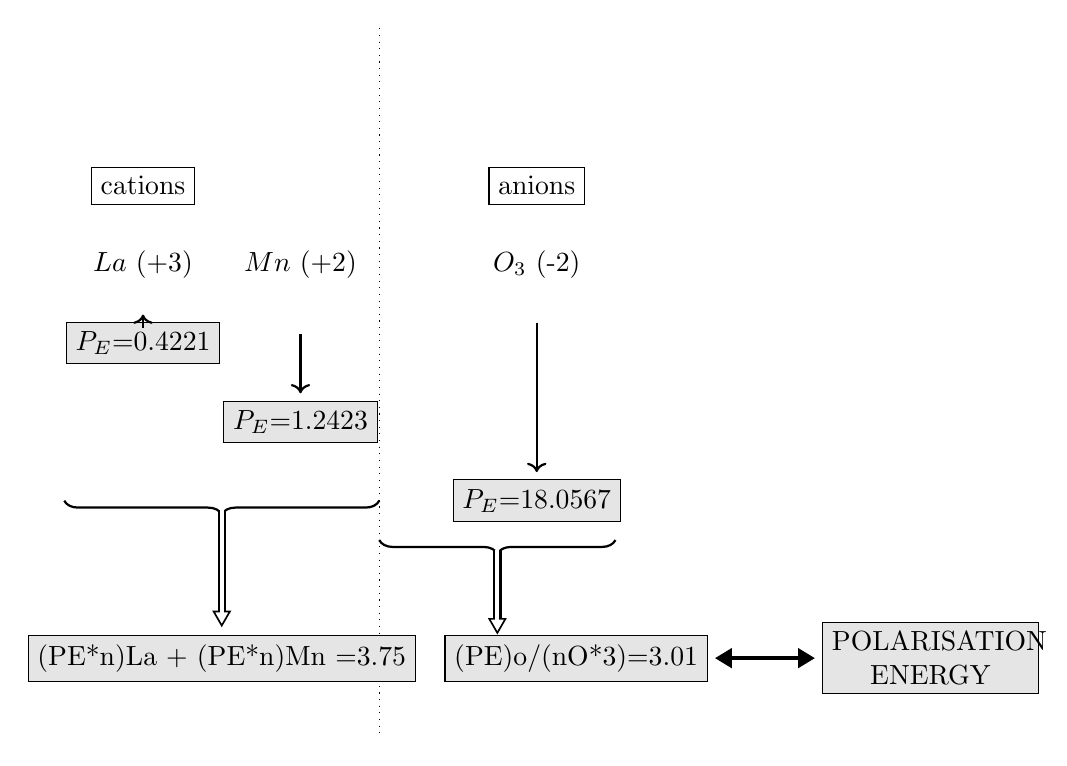
\begin{tikzpicture}
%\draw node{cations};
\node[rectangle,minimum size=0.01\textwidth,draw=black] (v1) at (0,0) {cations};
\node[rectangle,draw=black] (v2) at (5,0) {anions};
\node[circle] (E1) at (0,-1) {$La$ (+3)};
\node[circle] (E2) at (2,-1) {$Mn$ (+2)};
\node[circle] (E3) at (5,-1) {$O_3$ (-2)};
\tikzstyle{edge}=[->,thick]
\tikzstyle{arrow} = [ very thick, color=black, <->, >=Triangle]
%\tikzstyle{line}=[draw,thick]
%\tikzstyle{edge1}=[$\underbrace$,thick]
\tikzstyle{block} = [draw,rectangle,fill=black!10,minimum size=0.005,outer sep=1mm,text centered,minimum height=2mm]
%\node[rectangle](PE) at (0,-2) {$0.4221$};
\node[block](PE1) at (0,-2) {$P_E$=0.4221};
\draw[edge](E1)--(PE1);
\node[block,minimum size=1mm](PE2) at (2,-3) {$P_E$=1.2423};
\draw[edge](E2)--(PE2);
\node[block](PE3) at (5,-4) {$P_E$=18.0567};
\draw[edge](E3)--(PE3);
\node[block,text width=2.5cm](F4) at (10,-6) { POLARISATION ENERGY };
%\node[below=1cm](E1) {La};
%\node[below=1cm
%\node[circle,draw=black] (v1) at (0,0) {La};
%\tikzstyle{vertex} = [square]
%\node[vertex](v2)at(2,0){Mn};
%\draw[edge1](PE1)--(PE2);
\draw[decorate,thick,decoration={brace,amplitude=5pt,mirror}] 
(-1,-4) -- 
(3,-4){}; 
\draw (1,-4pt) coordinate (t_k)  {};
\node(B1) at (1,-4){};
\node(B2) at (4.5,-4.5){};
\draw[dotted](3,2)--(3,-7);
\draw[decorate,thick,decoration={brace,amplitude=5pt,mirror}] 
(3,-4.5) -- 
(6,-4.5){};
\node[block,minimum size=1mm](F1) at (1,-6) {(PE*n)La + (PE*n)Mn  =3.75};
\node[block,right of=F1](F2) at (4.5,-6) {(PE)o/(nO*3)=3.01};
\tikzstyle{vecArrow} = [thick, decoration={markings,mark=at position
	1 with {\arrow[semithick]{open triangle 60}}},
double distance=1.4pt, shorten >= 5.5pt,
preaction = {decorate},
postaction = {draw,line width=1.4pt, white,shorten >= 4.5pt}]
\draw[vecArrow] (B1) to (F1);
\draw[vecArrow] (B2) to (4.5,-5.7);
\draw[arrow] (F2.east) to (F4.west);
%  \path{vecArrow}(F2)--(F4);
%\framebox[0.5\textwidth][l]{n= (+3)     \hspace{1 cm}  (+2) \hspace{4 cm} (-2)} 
%\framebox[0.5\textwidth][l]{La    \hspace{2 cm}  Mn \hspace{4 cm} $O_3$} 
\end{tikzpicture}

}


\subsection{Selection Criteria}
Subsection text here.
\begin{enumerate}
	\item{Derived Radius values: The derived radius values can be used to conclude the cation and the anion required for the MA by matching their atomic radii to the derived values}
	\item {$P_o $ Parameter ,Based on the matching of the atomic radii , we can add the $P_o$ values such that $\sum {P_o}_{cations} = \sum {P_o}_{anion}$ }. Based on this , we can select multiple cations for the sample.
	\item{2.In case of mixed oxides , the mole fraction ratio of each cation or oxide compound can be derived as :-
		CALCULATION FOR THE MOLAR RATIO :-
		Depending on the ratio of the polarizability of the cation to anion , we can have the estimated molar fraction as
		\begin{equation}
		m = \frac{N_a X {r_a}^3}{N_c X {r_c}^3}
		\end{equation}
		
		Using the above derived values of the radius and the molar ratio calculation, we concluded for $Ga_2 O_3$
		with $m = 0.04$ }
	\item{In case of special crystal structures like pervoskite , spinel , fluorite , the radius ratio of the cation to anion has to be matched with the specified crystal requirement viz. }
\end{enumerate}



Subsubsection text here.


% An example of a floating figure using the graphicx package.
% Note that \label must occur AFTER (or within) \caption.
% For figures, \caption should occur after the \includegraphics.
% Note that IEEEtran v1.7 and later has special internal code that
% is designed to preserve the operation of \label within \caption
% even when the captionsoff option is in effect. However, because
% of issues like this, it may be the safest practice to put all your
% \label just after \caption rather than within \caption{}.
%
% Reminder: the "draftcls" or "draftclsnofoot", not "draft", class
% option should be used if it is desired that the figures are to be
% displayed while in draft mode.
%
%\begin{figure}[!t]
%\centering
%\includegraphics[width=2.5in]{myfigure}
% where an .eps filename suffix will be assumed under latex, 
% and a .pdf suffix will be assumed for pdflatex; or what has been declared
% via \DeclareGraphicsExtensions.
%\caption{Simulation Results}
%\label{fig_sim}
%\end{figure}

% Note that IEEE typically puts floats only at the top, even when this
% results in a large percentage of a column being occupied by floats.


% An example of a double column floating figure using two subfigures.
% (The subfig.sty package must be loaded for this to work.)
% The subfigure \label commands are set within each subfloat command, the
% \label for the overall figure must come after \caption.
% \hfil must be used as a separator to get equal spacing.
% The subfigure.sty package works much the same way, except \subfigure is
% used instead of \subfloat.
%
%\begin{figure*}[!t]
%\centerline{\subfloat[Case I]\includegraphics[width=2.5in]{subfigcase1}%
%\label{fig_first_case}}
%\hfil
%\subfloat[Case II]{\includegraphics[width=2.5in]{subfigcase2}%
%\label{fig_second_case}}}
%\caption{Simulation results}
%\label{fig_sim}
%\end{figure*}
%
% Note that often IEEE papers with subfigures do not employ subfigure
% captions (using the optional argument to \subfloat), but instead will
% reference/describe all of them (a), (b), etc., within the main caption.




% Note that IEEE does not put floats in the very first column - or typically
% anywhere on the first page for that matter. Also, in-text middle ("here")
% positioning is not used. Most IEEE journals use top floats exclusively.
% Note that, LaTeX2e, unlike IEEE journals, places footnotes above bottom
% floats. This can be corrected via the \fnbelowfloat command of the
% stfloats package.



\section{Conclusion}
The conclusion goes here.





% if have a single appendix:
%\appendix[Proof of the Zonklar Equations]
% or
%\appendix  % for no appendix heading
% do not use \section anymore after \appendix, only \section*
% is possibly needed

% use appendices with more than one appendix
% then use \section to start each appendix
% you must declare a \section before using any
% \subsection or using \label (\appendices by itself
% starts a section numbered zero.)
%


%\appendices
%\section{Proof of the First Zonklar Equation}
%Appendix one text goes here.

% you can choose not to have a title for an appendix
% if you want by leaving the argument blank
%\section{}
%Appendix two text goes here.


% use section* for acknowledgement
\section*{Acknowledgment}


The authors would like to thank...


% Can use something like this to put references on a page
% by themselves when using endfloat and the captionsoff option.
\ifCLASSOPTIONcaptionsoff
  \newpage
\fi



% trigger a \newpage just before the given reference
% number - used to balance the columns on the last page
% adjust value as needed - may need to be readjusted if
% the document is modified later
%\IEEEtriggeratref{8}
% The "triggered" command can be changed if desired:
%\IEEEtriggercmd{\enlargethispage{-5in}}

% references section

% can use a bibliography generated by BibTeX as a .bbl file
% BibTeX documentation can be easily obtained at:
% http://www.ctan.org/tex-archive/biblio/bibtex/contrib/doc/
% The IEEEtran BibTeX style support page is at:
% http://www.michaelshell.org/tex/ieeetran/bibtex/
\bibliographystyle{IEEEtran}
% argument is your BibTeX string definitions and bibliography database(s)
\bibliography{References}
%
% <OR> manually copy in the resultant .bbl file
% set second argument of \begin to the number of references
% (used to reserve space for the reference number labels box)
%\begin{thebibliography}{1}

%\bibitem{IEEEhowto:kopka}
%H.~Kopka and P.~W. Daly, \emph{A Guide to \LaTeX}, 3rd~ed.\hskip 1em plus
 % 0.5em minus 0.4em\relax Harlow, England: Addison-Wesley, 1999.

%\end{thebibliography}

% biography section
% 
% If you have an EPS/PDF photo (graphicx package needed) extra braces are
% needed around the contents of the optional argument to biography to prevent
% the LaTeX parser from getting confused when it sees the complicated
% \includegraphics command within an optional argument. (You could create
% your own custom macro containing the \includegraphics command to make things
% simpler here.)
%\begin{biography}[{\includegraphics[width=1in,height=1.25in,clip,keepaspectratio]{mshell}}]{Michael Shell}
% or if you just want to reserve a space for a photo:

%\begin{IEEEbiography}{Michael Shell}
%Biography text here.
%\end{IEEEbiography}

% if you will not have a photo at all:
%\begin{IEEEbiographynophoto}{John Doe}
%Biography text here.
%\end{IEEEbiographynophoto}

% insert where needed to balance the two columns on the last page with
% biographies
%\newpage

%\begin{IEEEbiographynophoto}{Jane Doe}
%Biography text here.
%\end{IEEEbiographynophoto}

% You can push biographies down or up by placing
% a \vfill before or after them. The appropriate
% use of \vfill depends on what kind of text is
% on the last page and whether or not the columns
% are being equalized.

%\vfill

% Can be used to pull up biographies so that the bottom of the last one
% is flush with the other column.
%\enlargethispage{-5in}



% that's all folks
\end{multicols}
\end{document}


